% Based on a a work of Dario Taraborelli

%!TEX TS-program = xelatex
%!TEX encoding = UTF-8 Unicode

\documentclass[10pt, a4paper]{article}
\usepackage{fontspec} 

% DOCUMENT LAYOUT
\usepackage{geometry} 
\geometry{a4paper, textwidth=4.5in, textheight=9.3in, marginparsep=20pt, marginparwidth=2in}
%\usepackage[top=3cm, bottom=3.5cm, outer=4cm, inner=4cm, heightrounded, textwidth=5cm, marginparwidth=2.5cm, marginparsep=1cm]{geometry}
\setlength\parindent{0in}

% FONTS
\usepackage[usenames,dvipsnames]{color}
\usepackage{xunicode}
\usepackage{xltxtra}
\defaultfontfeatures{Mapping=tex-text}
\setromanfont [Ligatures={Common}, Numbers={OldStyle}, Variant=01]{Calluna}
\setmonofont[Scale=.95]{Inconsolata}
\newfontfamily\unicodefont [Ligatures={Common}, Numbers={OldStyle}, Variant=01]{Adobe Garamond Pro}
\linespread{1.13}

% ---- CUSTOM COMMANDS
% \chardef\&="E050
\newcommand{\html}[1]{\href{#1}{\scriptsize\textsc{[html]}}}
\newcommand{\pdf}[1]{\href{#1}{\scriptsize\textsc{[pdf]}}}
\newcommand{\doi}[1]{\href{#1}{\scriptsize\textsc{[doi]}}}
% ---- MARGIN YEARS
\usepackage{marginnote}
\newcommand{\amper{}}{\chardef\amper="E0BD }
\newcommand{\years}[1]{\marginnote{\small #1}}
\renewcommand*{\raggedrightmarginnote}{}
%\setlength{\marginparsep}{25pt}
\reversemarginpar

% LISTS
\usepackage{enumitem}
\setitemize{noitemsep,topsep=0pt,parsep=0pt,partopsep=0pt,after=\vspace{1\baselineskip},before=\vspace{-.4\baselineskip}}

% HEADINGS
\usepackage{sectsty} 
\usepackage[normalem]{ulem} 
\sectionfont{\mdseries\upshape\Large}
\subsectionfont{\mdseries\scshape\normalsize} 
\subsubsectionfont{\mdseries\upshape\large}

% PDF SETUP
% ---- FILL IN HERE THE DOC TITLE AND AUTHOR
\usepackage[bookmarks, colorlinks, breaklinks, 
% ---- FILL IN HERE THE TITLE AND AUTHOR
	pdftitle={Albert Einstein - vita},
	pdfauthor={My name},
	pdfproducer={http://nitens.org/taraborelli/cvtex}
]{hyperref}  
\hypersetup{linkcolor=blue,citecolor=blue,filecolor=black,urlcolor=MidnightBlue} 

% DOCUMENT
\begin{document}
{\LARGE Antonio Piu}\\[.9cm]
Via Matteotti, 5\\
08020 Oniferi, Nuoro --- Italy\\[.3cm]
Mobile \texttt{(+39) 340-809-4307}\\[.3cm]
Email \href{mailto:antonio.piu@gmail.com}{antonio.piu@gmail.com}\\
Portfolio \href{http://antoniopiu.com/}{http://antoniopiu.com}\\

\begin{figure}[htbp]
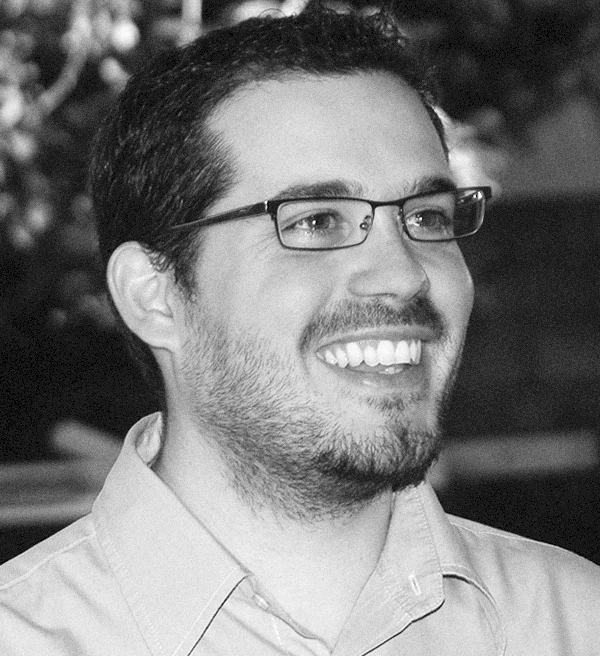
\includegraphics[height=5cm, width=5cm,keepaspectratio]{tessera-bn.jpg}
\end{figure}

%\vfill
\section*{Personal Information}
Birth date and place:  June 1st, 1982 --- Nuoro, Italy\\
Nationality:  Italian

%\hrule
\section*{Education {\unicodefont \emph{\&}} Learning}
\noindent
\years{2001-\emph{present}}University of Pisa, Italy\\
Facoltà di Ingegneria Informatica (Computer Engineering)\\
Bachelor's degree, 13 \emph{of} 16 exams achieved.\\[.4cm]
\years{1997-2001}Liceo Scientifico \emph{E. Fermi}, Nuoro, Italy\\
High School Diploma in Foreign Languages\\
100/100

%%\hrule
\section*{Current position}
\years{2012-\emph{present}}\textbf{Freelance professional}\\ 
Graphic design, front-end development, identity design, project management.\\

\begin{itemize}
\item Involved, as a project manager, in the specification and development \\of a web-based \emph{Intellectual Property} software.
\item Redesign of the websites network of a well-known italian Law Firm.
\item Graphic design for \href{http://papermine.com/}{Papermine}, a digital interactive magazine generator.
\item For more client work, please take a look at my \href{http://antoniopiu.com/}{online portfolio}.
\end{itemize}


%%\hrule
\section*{Professional Experience}
\years{2010-2012}\textbf{Studio FLU / Net7}\\ 
Via Marche 10, 56123 Pisa, Italy\\
Web and UI designer, front-end development.\\

\begin{itemize}
\item Design of websites and web application user interfaces.
\item \textsc{WordPress} and \textsc{Drupal} installation/configuration, theme development.
\item \textsc{w3c} Standard compliance and cross-browser testing.
\item Involved in projects for clients like \emph{Trussardi}, \emph{Prenatal}, \emph{Unicredit}.
\end{itemize}

\years{2008-2009}\textbf{Blackbit, Studio Associato}\\ 
Via Giordania 227, 58100 Grosseto, Italy\\
Web and UI designer, front-end development, identity {\unicodefont \emph{\&}} logo design.\\
\begin{itemize}
\item Design of websites and web applications \textsc{ui}.
\item Logo and stationery design for the Studio.
\end{itemize}

\years{2007-2008}\textbf{University of Pisa}\\ 
Department of Political Sciences, Via Serafini 3, 56126 Pisa\\
Design and implementation of a web portal using \textsc{Drupal}.\\

\years{2006-2007}\textbf{National Research Council (\textsc{cnr})}\\ 
Via Giuseppe Moruzzi 1, Pisa, Italy\\
Design and implementation of a website using \textsc{Drupal}.\\

\years{2004-2005}\textbf{Zeta Solution S.r.l.}\\ 
Via Giuntini 25, Navacchio di Cacina (\textsc{pi}), Italy\\
Print and digital graphic design and basic web development in \textsc{php}.\\

%%\hrule
\section*{Other skills {\unicodefont \emph{\&}} expertises}
\noindent
\years{Mothertongue}Italian\\
Sardinian\\[.4cm]
\years{Language skills} English -- Fluent spoken and written\\
Spanish -- Fluent spoken, good knowledge written\\
German -- Basic knowledge\\
French -- Basic knowledge\\[.4cm]
\years{Technical} Adobe\textregistered Photoshop\textregistered, Adobe\textregistered Illustrator\textregistered, \textsc{html}, \textsc{css} (professional proficiency)\\ 
JavaScript, \textsc{php} (intermediate knowledge)\\[.4cm]
\years{Driver's licence} Category \textsc{B}\\

\null
\vfill
\begin{center}
{\scriptsize  Last updated: \today\-\hspace{3pt} ·\-\hspace{3pt} 
Typeset in \fontspec{Times New Roman}\XeTeX}
\end{center}
\end{document}